\documentclass[../DefinizioneDiProdotto.tex]{subfiles}
\begin{document}
\section{Diagrammi di Sequenza}
Vengono qui riportati i diagrammi di sequenza delle operazioni principali dell'applicazione.
\subsection{Server Generazione Codice}
Di seguito viene riportato il diagramma di sequenza relativo al funzionamento del server per quanto riguarda la generazione del codice.\\
In questo diagramma possiamo notare che in seguito alla chiamata ascincrona di generazione del codice da parte del client il Main  provvede a inoltrare la richiesta al Request Handler il quale, tramite il CodeGenerator, richiama in ordine:
\begin{itemize}
	\item Parser;
	\item Coder;
	\item Builder;
	\item Zipper.
\end{itemize} 
Infine lo zip contenente il codice viene inviato al client.

\begin{figure}[H]\label{fig:Server}
	\centering
	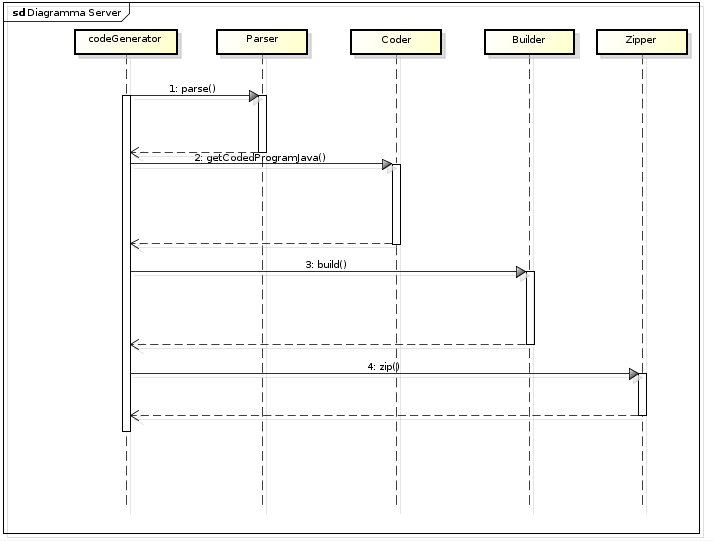
\includegraphics[scale=0.46]{Immagini/DiagrammaCodice.png}
	\caption{Server Generazione Codice}
\end{figure}


\subsection{Richiesta Generazione Codice}
Di seguito viene riportato il diagramma di sequenza relativo alla richiesta di generazione di codice,in questo caso Java, da parte di un'utente.\\
Per generare il codice l'utente clicca su "Genera Codice Java" innescando un'evento nella titlebarView.
La titlebarView richiama il requestHandler del client che invia la richiesta al Main del server.\\
Dal Main la richiesta viene inoltrata al requestHandler il quale richiama il CodeGenerator che si occupa della generazione del codice.

\begin{figure}[H]\label{fig:RichiestaGenerazione}
	\centering
	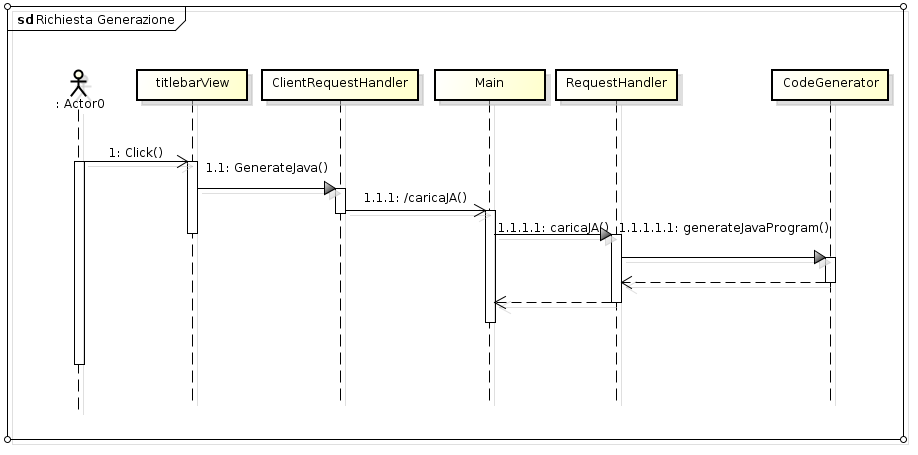
\includegraphics[scale=0.46]{Immagini/RichiestaGenerazione.png}
	\caption{Richiesta Generazione}
\end{figure}

\subsection{Salvataggio Progetto}
Di seguito viene riportato il diagramma di sequenza relativo alla richiesta di salvataggio del progetto corrente.\\
Per generare il codice l'utente clicca su "Salva" innescando un'evento nella titlebarView.\\
Successivamente vengono chiamate in successione metodi delle seguenti classi
\begin{itemize}
	\item dataManager: il metodo save() che si occupa di creare il file JSON una volta ottenuta lo schema corrente dal projectManager;
	\item projectModel: il metodo saveCurrentDiagram() che fornisce lo schema attuale al dataManager;
	\item project: il metodo getClassIndex() che restituisce una classe a partire dall'id richiesto.
\end{itemize}

\begin{figure}[H]\label{fig:Salvataggio}
	\centering
	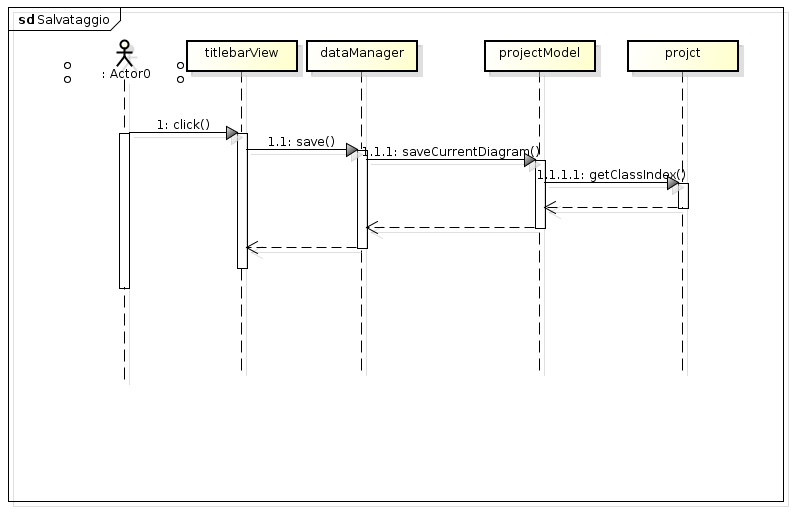
\includegraphics[scale=0.46]{Immagini/salvataggio.png}
	\caption{Salvataggio}
\end{figure}


\end{document} 